\chapter{Grundlagen} 
Im Kapitel Grundlagen erfolgt eine fachliche Beschreibung 
des Einsatzumfelds der Software. Dabei wird der Ablauf eines 
Rettungseinsatzes sowie die vorhandenen medizinischen Geräte erläutert. 
Im Anschluss werden die Komponenten der Software näher betrachtet, insbesondere
unter Berücksichtigung der verwendeten Technologien und Frameworks.

\section{Aufbau Rettungsdiensteinsatz}
Ein Rettungsdiensteinsatz in Deutschland beginnt mit einem Notruf bei der
Notrufnummer 112 oder der örtlichen Rettungsleitstelle. Die Leitstelle
entscheidet über die Art des Einsatzes und alarmiert die entsprechenden
Rettungsmittel. Zwei wichtige Komponenten des Rettungsdienstes sind dabei
das \ac{NEF} und der \ac{RTW}.
Das \ac{NEF}, besetzt mit einem Notarzt und oft auch einem Rettungsassistenten
oder Notfallsanitäter, hat die Aufgabe, den Notarzt so schnell wie möglich
zum Einsatzort zu bringen, um eine qualifizierte medizinische Versorgung
sicherzustellen. Parallel dazu wird der \ac{RTW}, in der Regel besetzt mit
Rettungsassistenten oder Notfallsanitätern, zum Einsatzort geschickt.
Der RTW übernimmt primär den Transport von Patienten. \\

Am Einsatzort erfolgt eine enge Zusammenarbeit zwischen dem Notarzt
und dem Notfallsanitäter im \ac{RTW}.Der Notfallsanitäter übernimmt die 
Erstversorgung des Patienten und bereitet alles für den Transport vor.
Der Notarzt unterstützt den Notfallsanitäter und übernimmt die
medizinische Verantwortung. Die Zusammenarbeit basiert auf klaren
Handlungsanweisungen und Protokollen. \\

Nach der Erstversorgung entscheiden Notarzt und Notfallsanitäter
gemeinsam über den weiteren Transport des Patienten, entweder zur nächsten
geeigneten Klinik oder zu einer spezialisierten Einrichtung, wenn erforderlich.
Die Abstimmung zwischen \ac{NEF} und \ac{RTW} sowie die Koordination zwischen Notarzt
und Notfallsanitäter sind entscheidend, um eine optimale Patientenversorgung
zu gewährleisten.\\

Der Ablauf eines Rettungsdiensteinsatzes beruht auf einer klaren Struktur
und effektiven Kommunikation, um in Notfallsituationen rasch und professionell
handeln zu können.\\

\section{Medizingeräte und Vitaldaten}
Die eingesetzte Medizintechnik am Einsatzort spielt 
eine entscheidende Rolle bei der Gewährleistung einer effizienten
und qualitativ hochwertigen präklinischen Versorgung von Patienten. 
Verschiedene medizinische Geräte und Instrumente werden gezielt eingesetzt, 
um eine schnelle Diagnosestellung, Stabilisierung des Patienten und die 
notwendigen lebenserhaltenden Maßnahmen zu ermöglichen.\\

Ein unverzichtbares Instrument ist der Defibrillator, der zur Behandlung
lebensbedrohlicher Herzrhythmusstörungen eingesetzt wird.\\

Zur medizinischen Ausstattung am Einsatzort gehören auch tragbare
Monitore zur kontinuierlichen Überwachung von Vitalparametern wie
Herzfrequenz, Blutdruck und Sauerstoffsättigung. Diese Informationen
sind entscheidend für die Einschätzung des Patientenzustands und die
Anpassung der therapeutischen Maßnahmen.\\

Aktuell verfügen die meisten dieser eingesetzten Geräte bereits
über hochperformante Datenschnittstellen, um die erfassten Informationen
an Dritte weiterzugeben. Dabei basieren die meisten Schnittstellen in der
Regel auf der Bluetooth-Technologie. Neuere Geräte setzen vermehrt auf
Cloud-Schnittstellen. In Kombination mit prioritisierten SIM-Karten werden
die Daten der Geräte so dezentral verteilt.\\

\section{Frontend Komponenten}
Die im Frontend eingesetzten Komponenten müssen den
anspruchsvollen Bedingungen im Einsatz standhalten und eine
benutzerfreundliche Bedienung für Rettungskräfte gewährleisten. 
Zusätzlich ist eine schnelle Austauschbarkeit im Falle eines Defekts
erforderlich, weshalb hochverfügbare Hardware notwendig ist. 
Aus diesem Grund wurde die Entscheidung getroffen, auf Consumer-Geräte 
zurückzugreifen, die zweifelsohne die zuvor genannten Kriterien erfüllen. 
Da die Geräte am Einsatzort ein essenzieller Bestandteil sind, um mit der 
\ac{TNA-Z} zu kommunizieren, wurde besonderer Wert auf hohe Flexibilität gelegt. 
Die Wahl fiel hier auf Apple- und Android-Telefone, die mit der in dieser Arbeit 
entwickelten Software bespielt werden. Zur Kostenoptimierung und schnelleren
Reaktion auf Änderungen wurde das Framework React Native gewählt. Zudem 
gewinnt Die plattformübergreifende Entwicklung zunehmend an akzeptanz in der Anwendungsentwicklung \cite{bertels2023kategorisierung}.\\

Für die Software des Notarztes, der sich an einem entfernten Ort befindet, 
wurde entschieden, eine Browseranwendung bereitzustellen. Der Vorteil einer
Browseranwendung liegt in der Entkopplung von der Hardware und der damit
verbundenen Flexibilität. Entschieden wurde sich für das Framework Next.js, u.a.
spielte auch die fachliche Nähe zu React Native eine entscheidende Rolle.\\

\subsection{React-Native}
React Native hat sich zu einer der führenden Plattformen für die
Entwicklung plattformübergreifender mobiler Anwendungen entwickelt. 
Durch die Nutzung von JavaScript/TypeScript und React ermöglicht es 
Entwicklern, hochperformante native Apps für iOS und Android zu erstellen. \\

Einer der Hauptvorteile von React Native ist die Fähigkeit, dass 
React Native JavaScript/TypeScript-Code in echten nativen Code komeliert.
Dadurch sehen und fühlen sich die erstellten Apps so an, als wären sie 
mit nativen Entwicklungstechnologien erstellt worden.\\

Ein weiteres entscheidendes Merkmal ist die Möglichkeit der 
Wiederverwendung von Code zwischen verschiedenen Plattformen.
Der Großteil des Codes kann plattformübergreifend verwendet werden,
was die Entwicklungseffizienz erheblich steigert und konsistente 
Funktionalitäten auf verschiedenen Geräten gewährleistet.\\

Die Architektur von React Native fördert die Modulstruktur, 
was bedeutet, dass verschiedene Funktionen in separate Module aufgeteilt 
werden können. Die React Native-Community hat eine breite Palette 
von vorgefertigten Modulen geschaffen, die den Entwicklungsprozess 
beschleunigen und den Funktionsumfang erweitern.\\

Der grundlegende Aufbau von React Native basiert auf React-Komponenten,
die Teile der Benutzeroberfläche repräsentieren und sowohl einfach
als auch komplex sein können. 
JSX, eine Syntaxerweiterung für JavaScript, wird verwendet, um Benutzeroberflächenelemente 
zu deklarieren, wodurch die Erstellung von UI-Komponenten auf eine 
intuitive Weise erfolgt.\\

\begin{figure}[H]
    \centering
    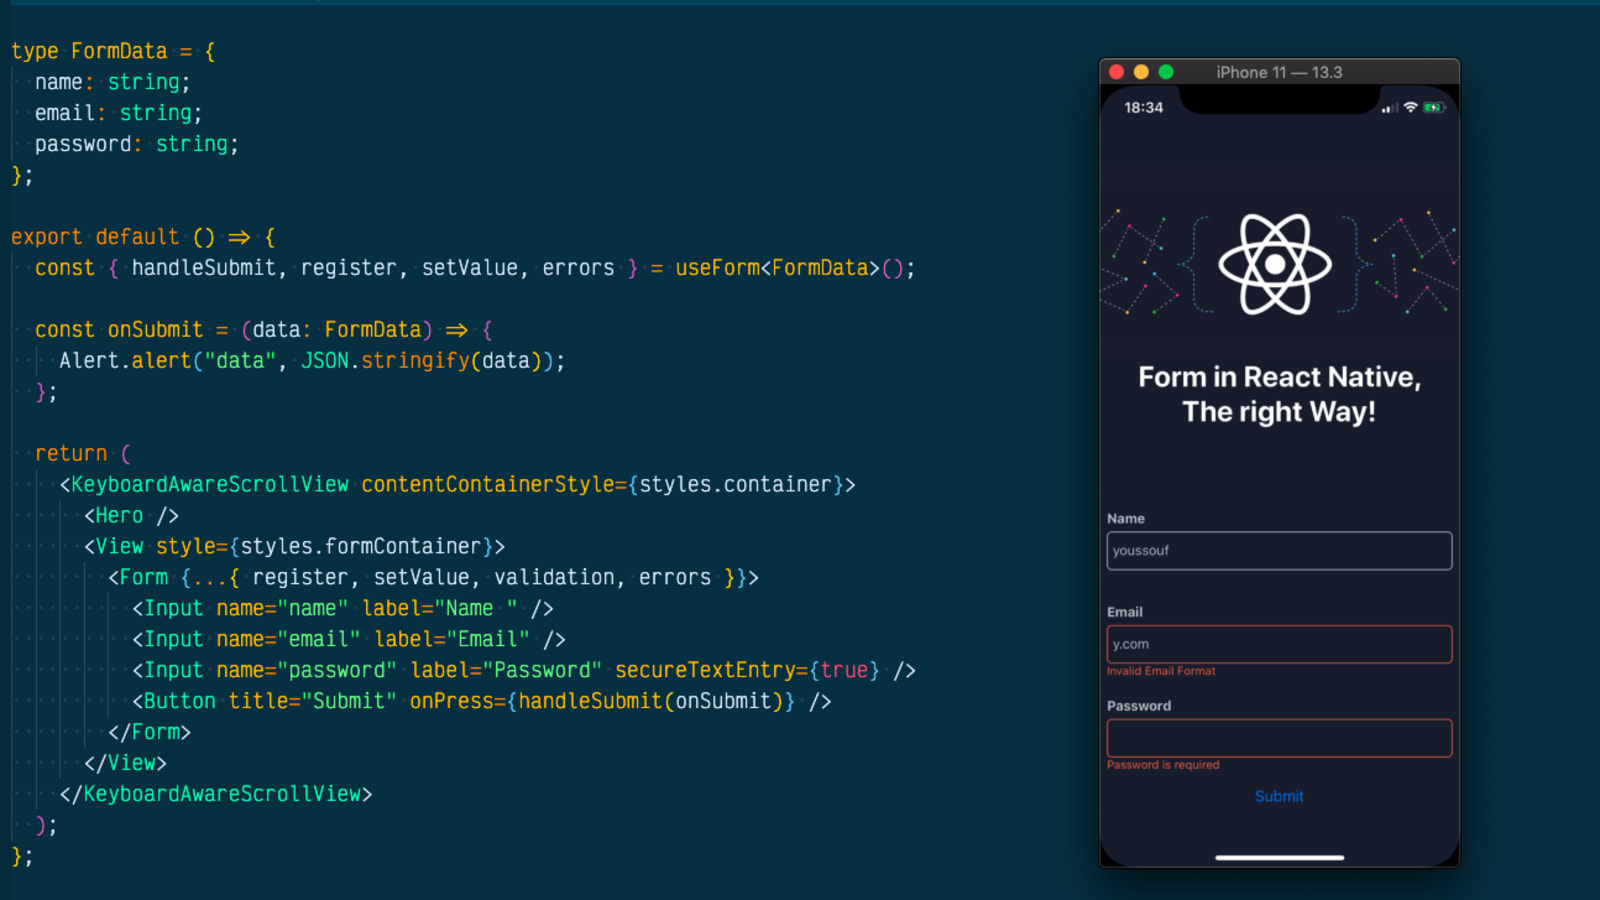
\includegraphics[width=1.0\textwidth]{ReactNative}
    \caption{Darstellung Code und UI mit React-Native[Quelle: \cite{ReactNativeCode}]}
    \label{img:ReactNative}
\end{figure}

Die Styling-Sprache in React Native ähnelt CSS, bietet jedoch nur eine 
begrenzte Menge an Styles. Dies stellt sicher, dass die Apps 
auf verschiedenen Plattformen konsistent aussehen, während 
gleichzeitig plattformspezifische Styles angewendet werden können.\\

\subsection{Next.js}
Lorem ipsum dolor sit amet, consetetur sadipscing
elitr, sed diam nonumy eirmod tempor invidunt ut labore
et dolore magna aliquyam erat, sed diam voluptua. At vero eos et
accusam et justo duo dolores et ea rebum. Stet clita kasd gubergren, 
no sea takimata sanctus est Lorem ipsum dolor sit amet. Lorem ipsum dolor 
sit amet, consetetur sadipscing elitr, sed diam nonumy eirmod tempor 
invidunt ut labore et dolore magna aliquyam erat, sed diam voluptua. 
At vero eos et accusam et justo duo dolores et ea rebum. Stet clita kasd 
gubergren, no sea takimata sanctus est Lorem ipsum dolor sit amet.

\section{Backend Komponenten}
Lorem ipsum dolor sit amet, consetetur sadipscing
elitr, sed diam nonumy eirmod tempor invidunt ut labore
et dolore magna aliquyam erat, sed diam voluptua. At vero eos et
accusam et justo duo dolores et ea rebum. Stet clita kasd gubergren, 
no sea takimata sanctus est Lorem ipsum dolor sit amet. Lorem ipsum dolor 
sit amet, consetetur sadipscing elitr, sed diam nonumy eirmod tempor 
invidunt ut labore et dolore magna aliquyam erat, sed diam voluptua. 
At vero eos et accusam et justo duo dolores et ea rebum. Stet clita kasd 
gubergren, no sea takimata sanctus est Lorem ipsum dolor sit amet.

\subsection{Microservices mit Java springboot}
Lorem ipsum dolor sit amet, consetetur sadipscing
elitr, sed diam nonumy eirmod tempor invidunt ut labore
et dolore magna aliquyam erat, sed diam voluptua. At vero eos et
accusam et justo duo dolores et ea rebum. Stet clita kasd gubergren, 
no sea takimata sanctus est Lorem ipsum dolor sit amet. Lorem ipsum dolor 
sit amet, consetetur sadipscing elitr, sed diam nonumy eirmod tempor 
invidunt ut labore et dolore magna aliquyam erat, sed diam voluptua. 
At vero eos et accusam et justo duo dolores et ea rebum. Stet clita kasd 
gubergren, no sea takimata sanctus est Lorem ipsum dolor sit amet.

\subsection{Authentifizierung}
Lorem ipsum dolor sit amet, consetetur sadipscing
elitr, sed diam nonumy eirmod tempor invidunt ut labore
et dolore magna aliquyam erat, sed diam voluptua. At vero eos et
accusam et justo duo dolores et ea rebum. Stet clita kasd gubergren, 
no sea takimata sanctus est Lorem ipsum dolor sit amet. Lorem ipsum dolor 
sit amet, consetetur sadipscing elitr, sed diam nonumy eirmod tempor 
invidunt ut labore et dolore magna aliquyam erat, sed diam voluptua. 
At vero eos et accusam et justo duo dolores et ea rebum. Stet clita kasd 
gubergren, no sea takimata sanctus est Lorem ipsum dolor sit amet.

\subsection{Kubernetes}
Lorem ipsum dolor sit amet, consetetur sadipscing
elitr, sed diam nonumy eirmod tempor invidunt ut labore
et dolore magna aliquyam erat, sed diam voluptua. At vero eos et
accusam et justo duo dolores et ea rebum. Stet clita kasd gubergren, 
no sea takimata sanctus est Lorem ipsum dolor sit amet. Lorem ipsum dolor 
sit amet, consetetur sadipscing elitr, sed diam nonumy eirmod tempor 
invidunt ut labore et dolore magna aliquyam erat, sed diam voluptua. 
At vero eos et accusam et justo duo dolores et ea rebum. Stet clita kasd 
gubergren, no sea takimata sanctus est Lorem ipsum dolor sit amet.

